%% ------------------------------------------------------------------------- %%
\chapter{Ubicación del punto láser}\index{Detección!del punto láser}
\label{cap:deteccion}
En este capítulo se detalla\ldots

\begin{figure}[h]
	\centering
	\begin{tabular}{cc}
		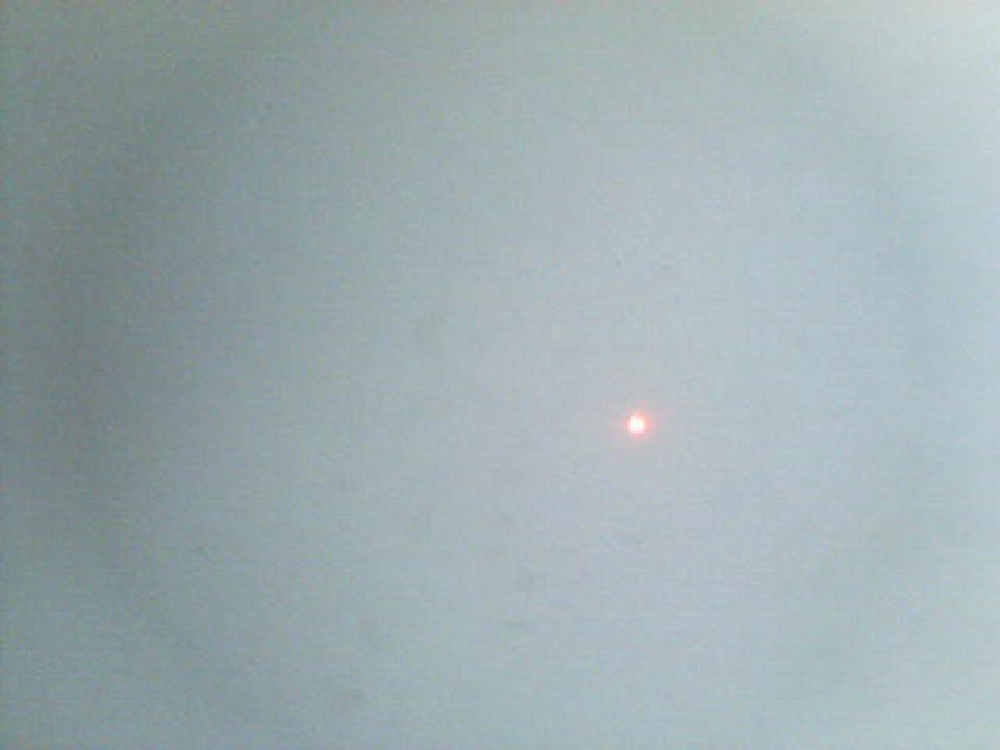
\includegraphics[width=0.4\textwidth]{Deteccion/Laser2.pdf} &
		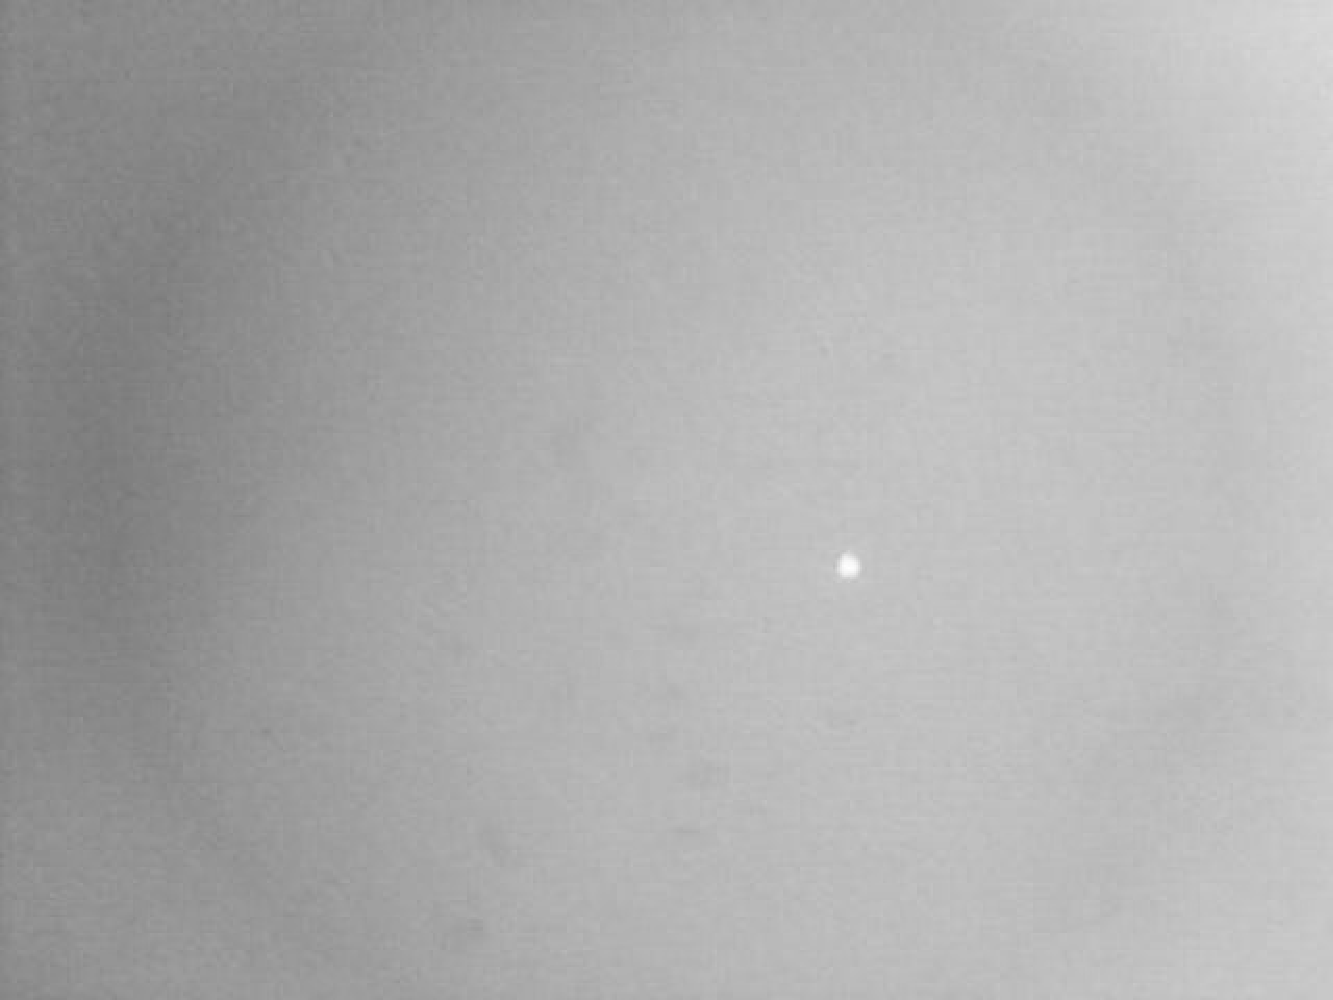
\includegraphics[width=0.4\textwidth]{Deteccion/Laser2_gray.pdf} \\
		    (a) & (b) \\
		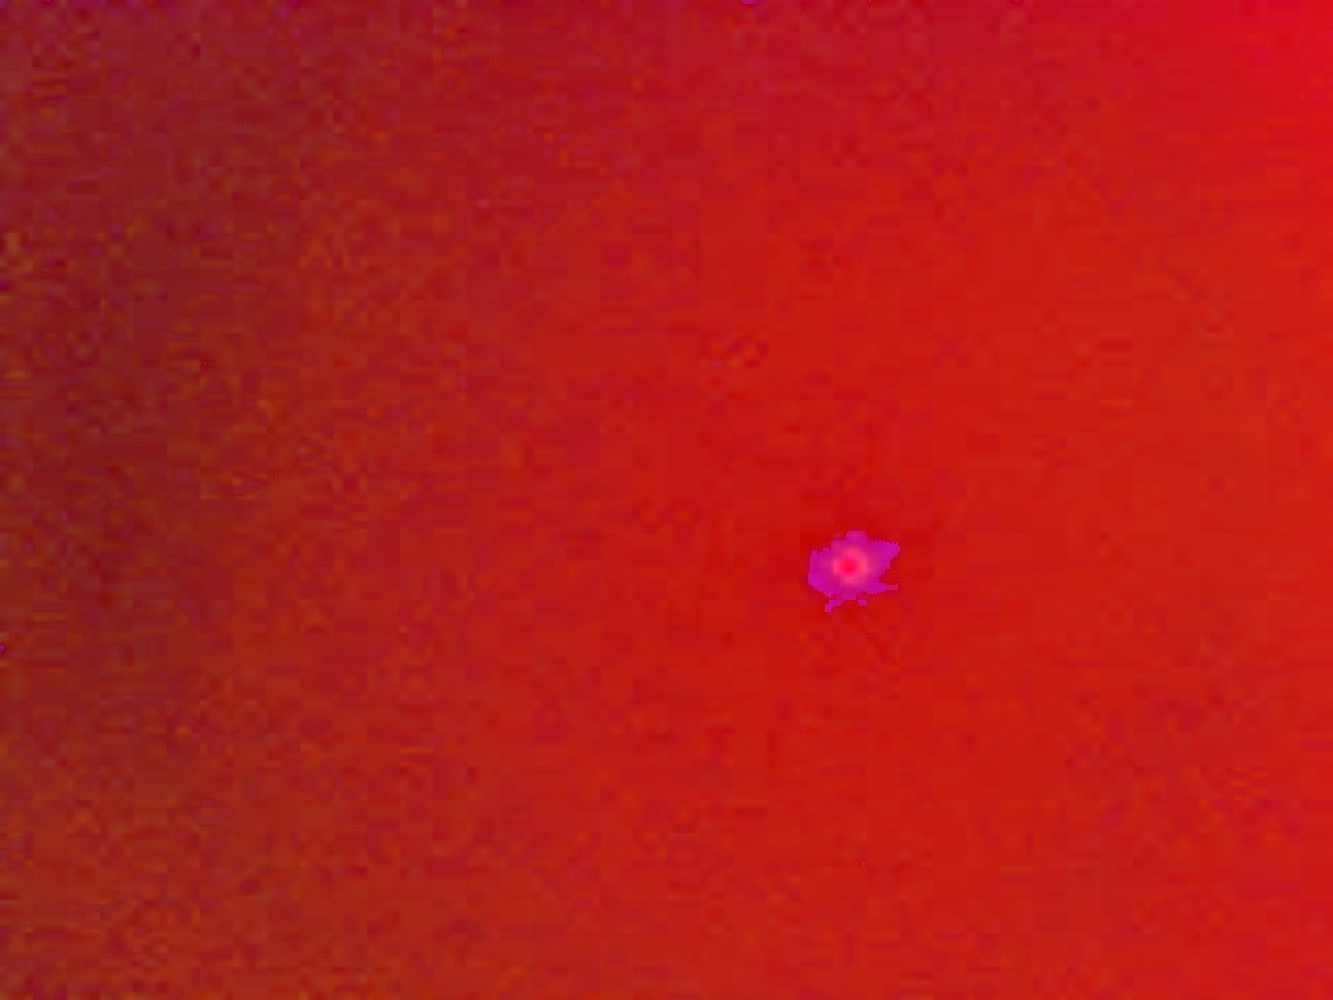
\includegraphics[width=0.4\textwidth]{Deteccion/Laser2_hsv.pdf} &
		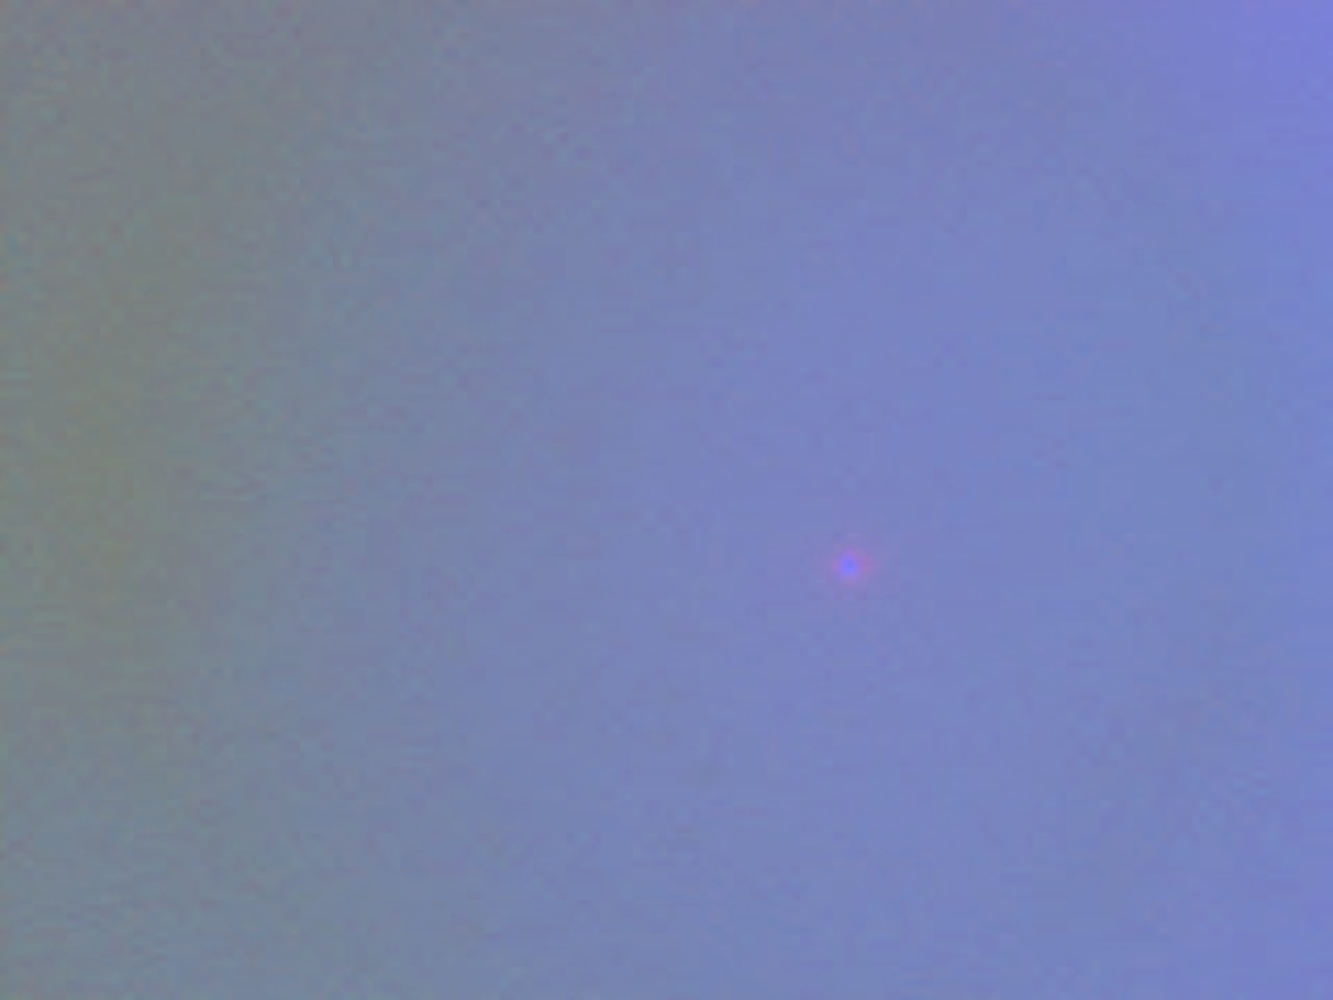
\includegraphics[width=0.4\textwidth]{Deteccion/Laser2_result.pdf} \\
		    (c) & (d)\\
	\end{tabular}
	\caption{Ejemplo de una imagen con doble fila y doble columna: 
	(a) Imagen en color RGB (b) Imagen en escala de grises (c) Imagen en escala de colores HSV 
	(d) Imagen en escala de colores Y'CbCr (Chrominance-Luminance)}
	\label{fig:filtroscolor}
\end{figure}

\section{Análisis y conclusiones}
En este capítulo se ha descrito\ldots


\algsetup{indent=2em}
\begin{algorithm}[t]

\begin{algorithmic}[1]
%\COMMENT{Imagen de 3 canales en formato YCrCb}
\REQUIRE Imagen en formato YCrCb de 3 canales  
%\COMMENT{La posición (x,y) del punto láser en la imagen en números enteros}
\ENSURE Posición (x,y)  .
\medskip
%aqui viene el algoritmo
\COMMENT{Se busca en la segunda mitad de la altura de la imagen}
\STATE$ limih = imagen \rightarrow altura/2;$
\COMMENT{Se busca en la sección 5 de la imagen, ver Figura\ldots}
\STATE $limiwinitial = imagen \rightarrow ancho/3;$
\STATE $limiwfinal = limiwinitial*2;$
\COMMENT{Para cada fila a partir de limih, buscamos desde limiwinitial hasta limiwfinal}
\FOR{$f=limih; f \leq imagen\rightarrow altura$}
\FOR{$c=limihinitial; c\leq limiwfinal$}
\STATE $suma= imagen[f][c].canal1 + imagen[f][c].canal2 + imagen[f][c].canal3;$
\IF{$suma > max $}
\STATE $max =suma;$
\STATE $x = c;$
\STATE $y = f;$
\ENDIF
\STATE $suma=0;$
\ENDFOR
\ENDFOR
\end{algorithmic}
\caption{Algoritmo de búsqueda de la posición (x,y) del reflejo del punto láser en la imagen digital.}
\label{alg:busquedaImagen}
\end{algorithm}	
	
